%\documentstyle[epsf,twocolumn]{jarticle}       %LaTeX2.09仕様
%\documentclass[twocolumn]{jarticle}     %pLaTeX2e仕様
\documentclass{jarticle}     %pLaTeX2e仕様

%一枚組だったら[twocolumn]関係のとこ消す

\setlength{\topmargin}{-45pt}
%\setlength{\oddsidemargin}{0cm} 
\setlength{\oddsidemargin}{-7.5mm}
%\setlength{\evensidemargin}{0cm} 
\setlength{\textheight}{24.1cm}
%setlength{\textheight}{25cm} 
\setlength{\textwidth}{17.4cm}
%\setlength{\textwidth}{172mm} 
\setlength{\columnsep}{11mm}

\kanjiskip=.07zw plus.5pt minus.5pt

\usepackage[dvipdfm]{graphicx}
\usepackage{ccaption}
\usepackage{algorithm}
\usepackage{algorithmic}
\usepackage{subcaption}
\usepackage{enumerate}
\usepackage{comment}
\usepackage{url}
\usepackage{multirow}
\usepackage{diagbox}
\usepackage{amssymb}
\usepackage{mathtools}
\usepackage{wrapfig}
\usepackage{graphicx}
\usepackage{float}
\usepackage{amsmath}
\usepackage{lipsum}


\begin{document}
  \noindent
  \hspace{1em}

  \today Creation班 ゼミ
  \hfill
  \ \  西村昭賢 

  \vspace{2mm}
  \hrule
  \begin{center}
  {\Large \bf 進捗報告}
  \end{center}
  \hrule
  \vspace{3mm}


\section{GPT4 の出力結果}
GPT 4 にカードプールを生成してもらい各役職のデッキを作成してもらった. 図 \ref{fig:deck1}, \ref{fig:deck2}, \ref{fig:deck3}, \ref{fig:deck4} に結果を示す.
また, 

\begin{figure}[ht]
  \centering
  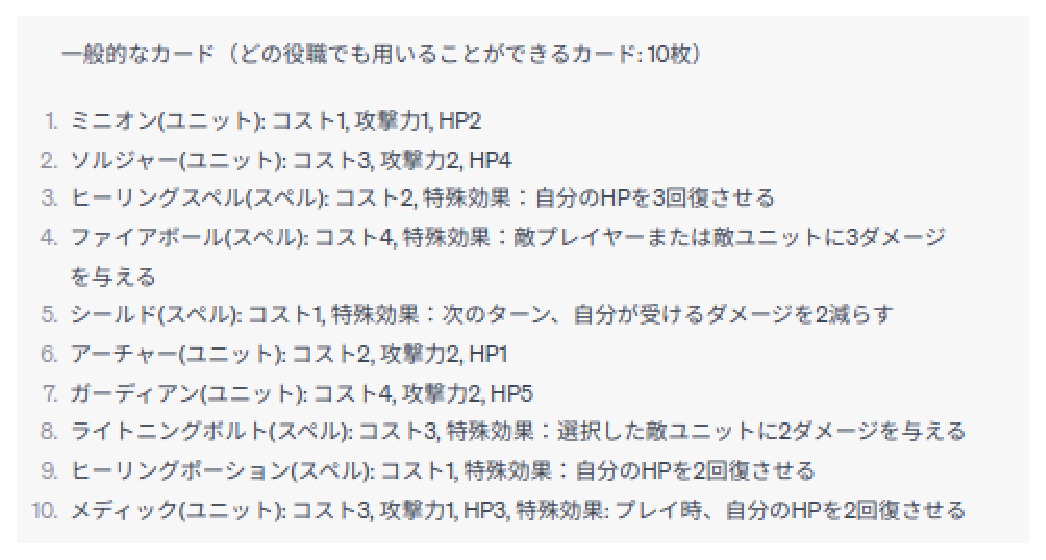
\includegraphics[width=120mm]{assets/1.eps}
  \vspace{-0.3cm}
  \caption{どの役職でも使えるカード}
  \label{fig:deck1}
\end{figure}


\begin{figure}[ht]
  \centering
  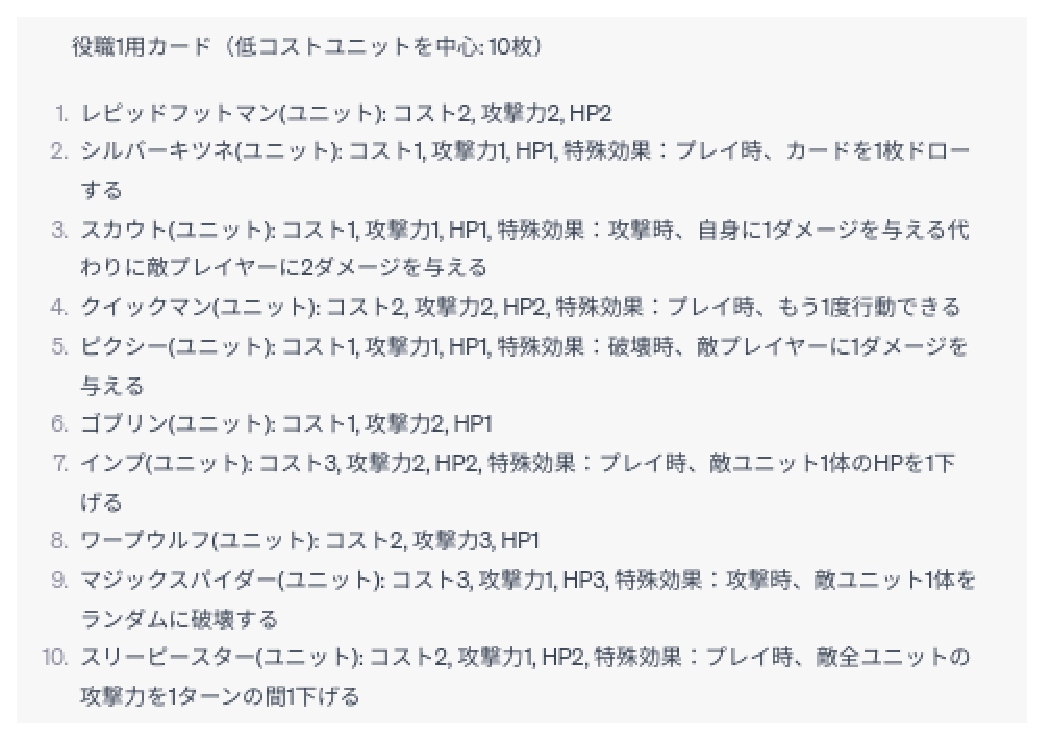
\includegraphics[width=120mm]{assets/2.eps}
  \vspace{-0.3cm}
  \caption{低コストユニット中心の役職専用のカード}
  \label{fig:deck2}
\end{figure}


\begin{figure}[ht]
  \centering
  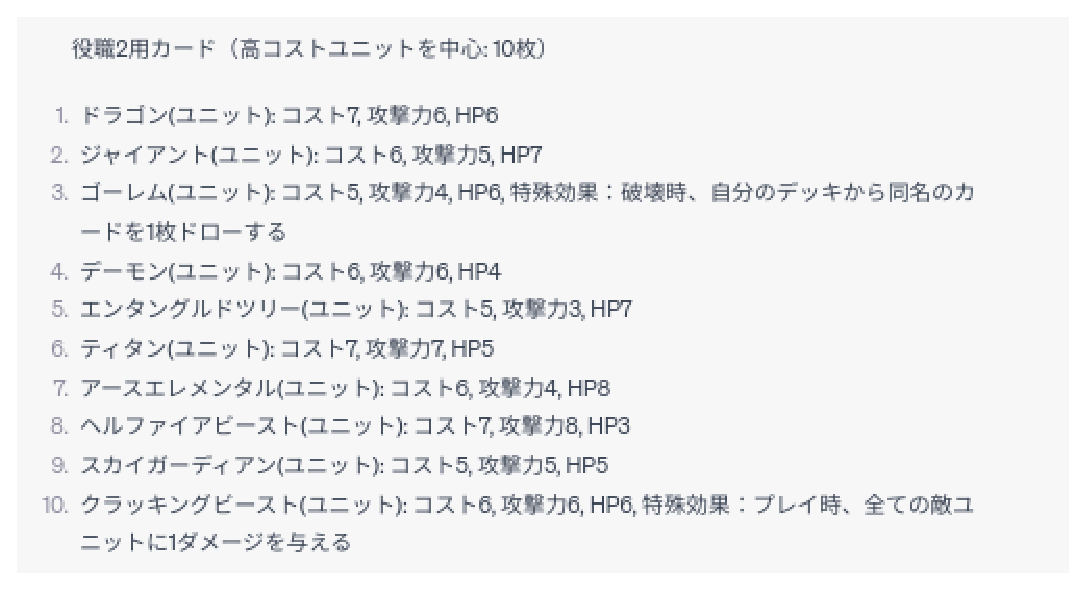
\includegraphics[width=120mm]{assets/3.eps}
  \vspace{-0.3cm}
  \caption{高コストユニット中心の役職専用のカード}
  \label{fig:deck3}
\end{figure}


\begin{figure}[ht]
  \centering
  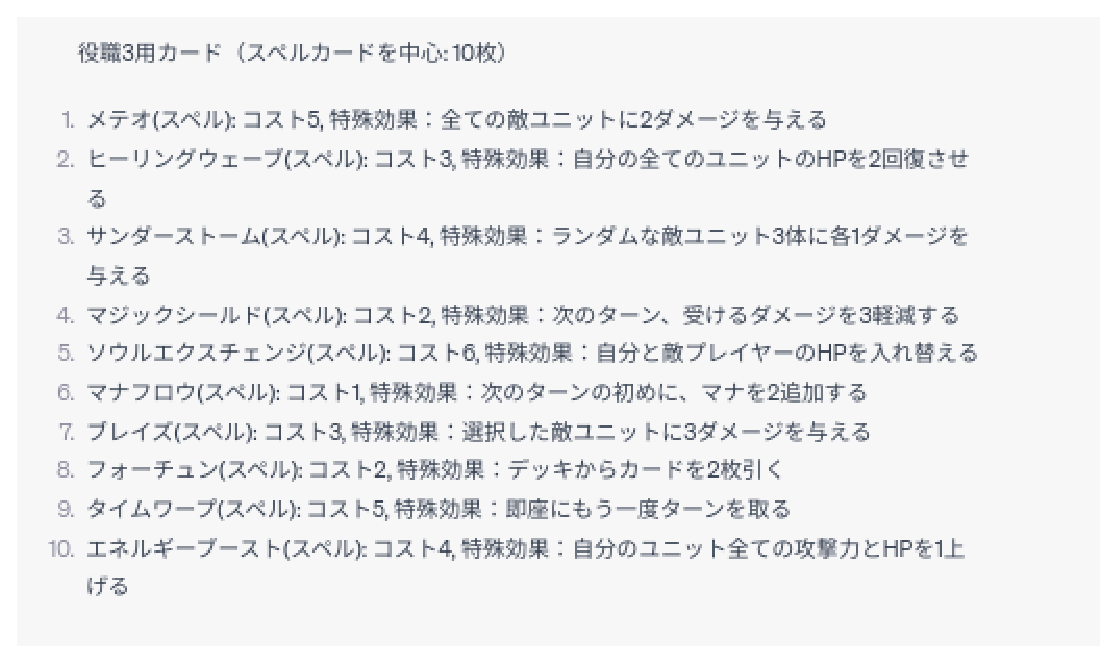
\includegraphics[width=120mm]{assets/4.eps}
  \vspace{-0.3cm}
  \caption{スペルカード中心の役職専用のカード}
  \label{fig:deck4}
\end{figure}

また, デッキの内訳も決めてもらった.
図 \ref{fig:deck5} に出力結果を示す.

\begin{figure}[ht]
  \centering
  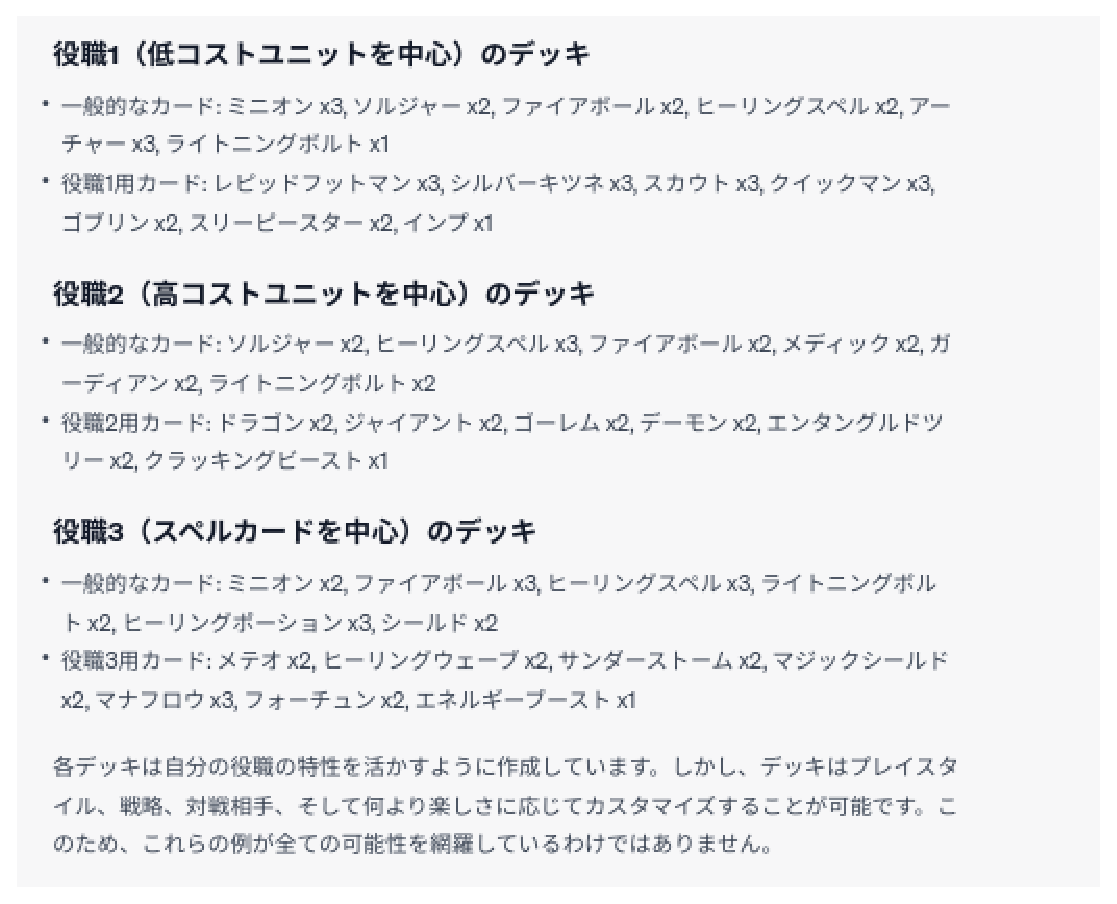
\includegraphics[width=120mm]{assets/5.eps}
  \vspace{-0.3cm}
  \caption{3 役職のデッキ編成}
  \label{fig:deck5}
\end{figure}


\section{数値実験}

図 \ref{fig:deck5} における低コストユニット中心の役職のカードとデッキを実装したため, 自己対戦で強化学習のみで戦略を構築する実験をした.

\begin{figure}[ht]
  \centering
  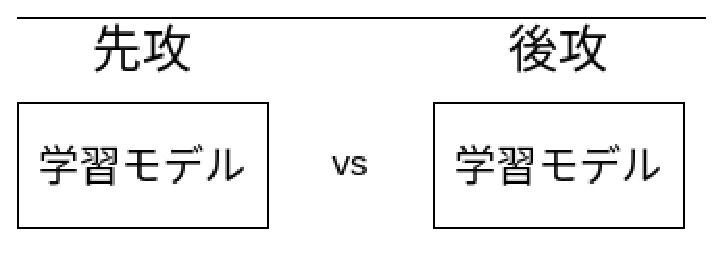
\includegraphics[width=120mm]{assets/training.eps}
  \vspace{-0.3cm}
  \caption{学習の様子}
  \label{fig:training}
\end{figure}

図 \ref{fig:training} に学習の様子を示す. 1つのモデルのインスタンスで学習をした.
図 \ref{fig:reawrd} に学習中の報酬の推移を示している.

結果として, Test 時の勝率が 0.0 \% となり, 恐らく何かしらのバグが発生している可能性があると考えられる.
急いで他のカードとバグの調査をします.

\begin{figure}[ht]
  \centering
  \includegraphics[width=120mm]{assets/self_play.eps}
  \vspace{-0.3cm}
  \caption{学習中の報酬の推移}
  \label{fig:reward}
\end{figure}

\begin{figure}[ht]
  \centering
  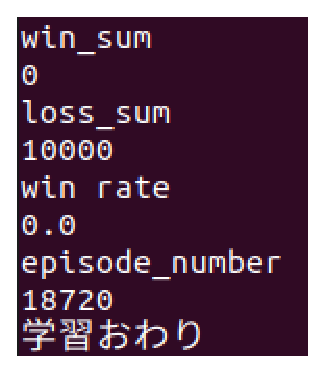
\includegraphics[width=120mm]{assets/result.eps}
  \vspace{-0.3cm}
  \caption{検証時の勝率 (恐らくバグ)}
  \label{fig:result}
\end{figure}


\section{見直すこと}
今回のバグの原因として考えられるのがスペルカードの導入です. 単体のテストはしていて問題はないはずなので DQN 側でなにか問題があると考えています. 
以前まではユニットのみ考えていたため, 行動空間や状態空間の定義をし直す必要があると考えています.
表 \ref{table:state}, \ref{table:action} に以前までのユニットのみの実験で用いていた状態空間と行動空間の定義を示します. 
\begin{table}[t]
  \small
  \centering
  \caption{定義した状態空間}
  \label{table:state}
  \vspace{-0.3cm}
  \scalebox{0.80}[0.80]{
    \begin{tabular}{|c|c|c|c|}
      \hline
      状態説明                        & 次元数        & 最小値        & 最大値         \\ \hline \hline
      各プレイヤーの HP & 2 & 0 & 20 \\ \hline
      各プレイヤーの マナ & 2 & 0 & 5 \\ \hline
      \begin{tabular}{c}
        手札 1 $\sim$ 9 の\\HP , 攻撃力, コスト, 特殊効果
        \end{tabular}      & 36         & 0          & 5          \\
      \hline
      \begin{tabular}{c}
        自盤面 1 $\sim$ 5 の\\HP と攻撃力
      \end{tabular}     & 10         & 0          & 5 \\
      \hline
      \begin{tabular}{c}
        敵盤面 1 $\sim$ 5 の\\HP と攻撃力
      \end{tabular}     & 10         & 0          & 5 \\
      \hline
      \begin{tabular}{c}
        自盤面 1 $\sim$ 5 が\\攻撃可能かどうか
      \end{tabular} & 5          & 0          & 1  \\
      \hline
      \begin{tabular}{c}
        お互いのデッキの\\残り枚数
      \end{tabular}     & 2 & 0 & 30 \\
       \hline
      \end{tabular}
  }
  \end{table}

  \begin{table}[t]
    \centering
    \caption{定義した行動空間}
    \vspace{-0.3cm}
    \label{table:action}
    \scalebox{0.80}[0.80]{
      \begin{tabular}{|c|c|}
        \hline
        行動説明                          & 次元数        \\ \hline \hline
        手札 1 $\sim$ 9 を自盤面にプレイ             & 9          \\ \hline
        自盤面 1 で敵盤面 1 $\sim$ 5 に攻撃or敵プレイヤーに攻撃    & 6          \\ \hline
        自盤面 2 で敵盤面 1 $\sim$ 5 に攻撃or敵プレイヤーに攻撃    & 6          \\ \hline
        自盤面 3 で敵盤面 1 $\sim$ 5 に攻撃or敵プレイヤーに攻撃    & 6          \\ \hline
        自盤面 4 で敵盤面 1 $\sim$ 5 に攻撃or敵プレイヤーに攻撃    & 6          \\ \hline
        自盤面 5 で敵盤面 1 $\sim$ 5 に攻撃or敵プレイヤーに攻撃    & 6          \\ \hline
        ターンエンド & 1 \\ \hline
        \end{tabular}
    }
      \end{table}
  
      \par
    また, 自己対戦では DQN を用いてきましたが, JSAI の際のぷよぷよの人が用いていた Unity ML-Agent が提供している self-play は PPO と SAC を混合させたような実装をしているようです.\cite{self} 
    まだ実装自体は見つけていませんが, 新しいアルゴリズムの実装も考えておきます.


%index.bibはtexファイルと同階層に置く
%ちゃんと\citeしないと表示されない(1敗)
\bibliography{index.bib}
\bibliographystyle{junsrt}

\end{document}